\chapter{相关技术方法概述}


本章就基于进化算法的FPGA脉动阵列布局所涉及的各方面技术进行总结与阐述。
首先总结经典的神经网络硬件加速设计,主要涉及基于线性缓存的卷积核设计与
高速脉动阵列。然后介绍FPGA的基本实现原理与RapidWright FPGA定制化
实现框架,最后介绍经典的几类FPGA布局算法与基本的进化算法。

\section{神经网络硬件加速}

随着人工智能的兴起,卷积神经网络在计算机视觉领域得到了大规模应用,比如图像分类~\cite{szegedy2017inception}、物体检测~\cite{redmon2018yolov3}、
语义分割~\cite{barkau1996unet}等诸多子领域。同时,因为卷积神经网络训练和预测中的计算需求和易于并行化的特点,在可编程硬件上实现
神经网络计算架构受到了广泛的研究关注。本节主要介绍两种经典的卷积神经网络加速器设计:
Line-Buffer型卷积计算单元~\cite{qiu2016going}与脉动阵列~\cite{nachiket_stc_fpl2019}。

\begin{figure}[h]
	\centering
	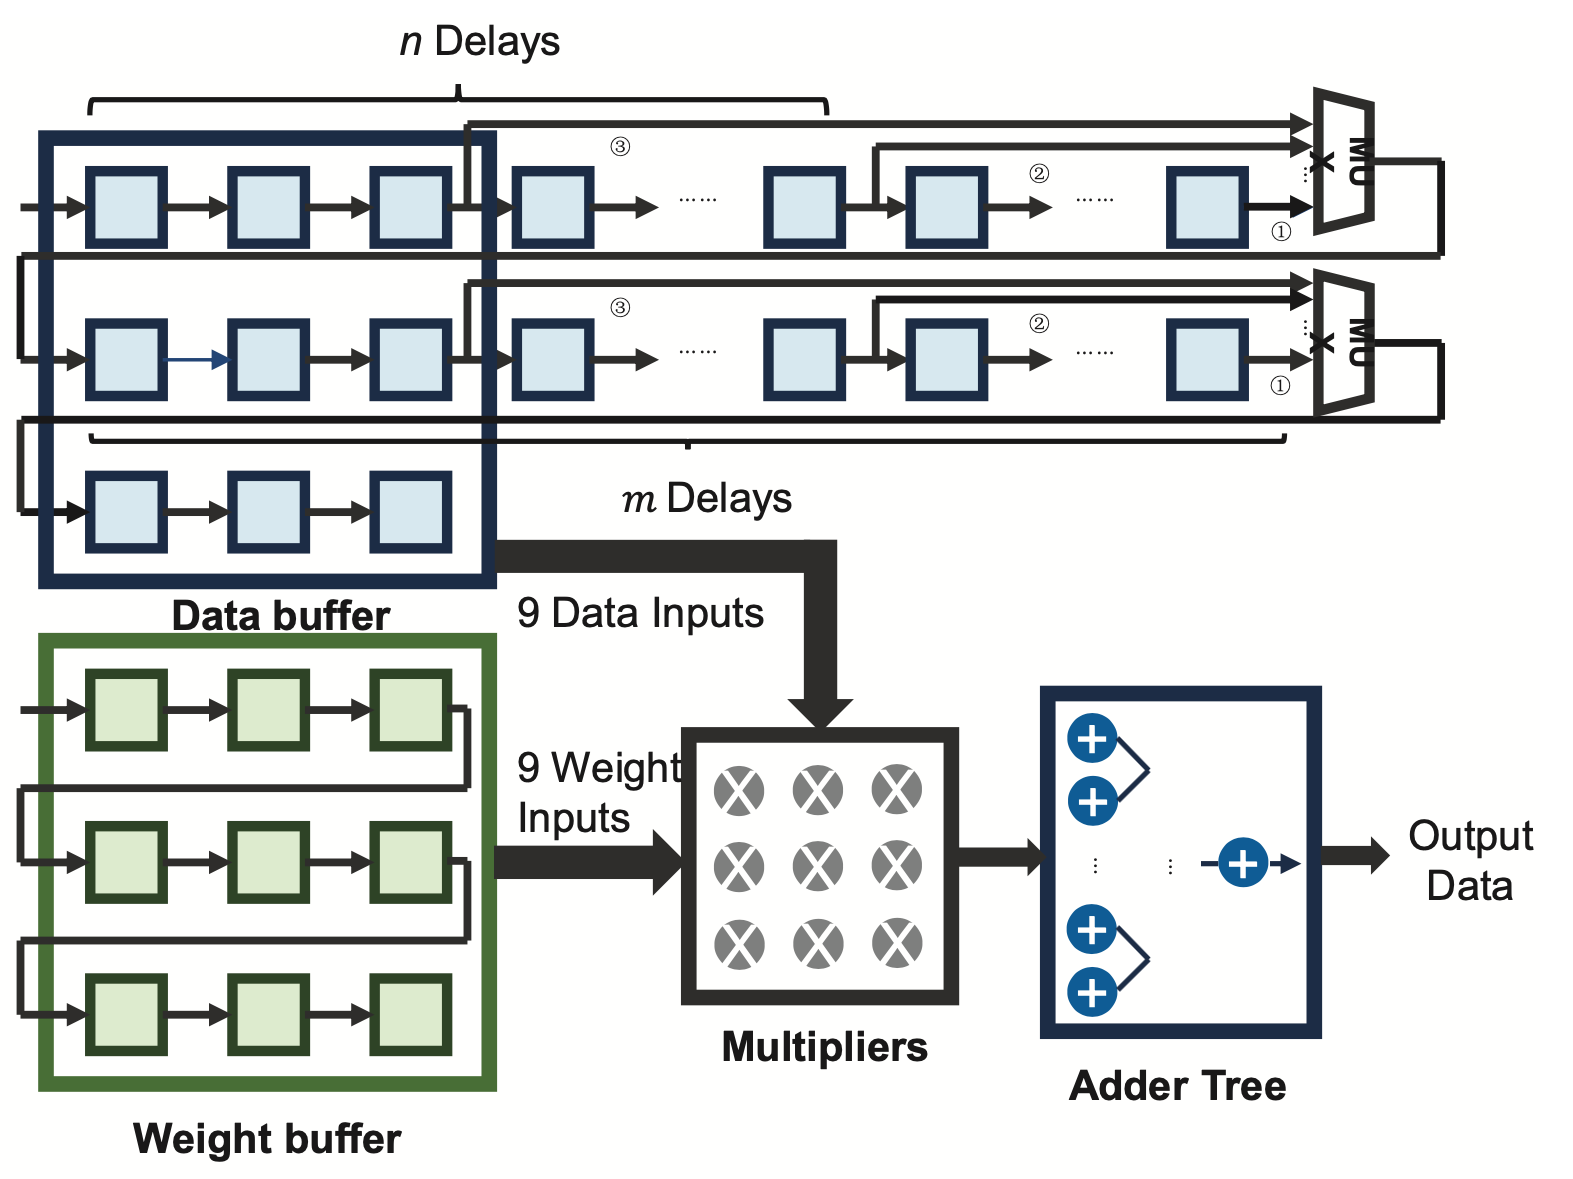
\includegraphics[width=0.8\textwidth]{figure/line-buffer}
	\caption{Line Buffer型卷积计算单元~\cite{qiu2016going}} 
	\label{fig:conv}
\end{figure}

如图\ref{fig:conv}所示为Line-Buffer型卷积计算单元的基本结构,其特点是使用移位寄存器
构成数据缓存器,通过不断输入像素数据完成等效的卷积滑窗操作。数据缓存器窗内的像素值与权重缓存器
内的权重值并行输入乘法器阵列。乘法器阵列的结果经过加法树并行累加得到一次卷积操作的结果。
Line-Buffer型卷积计算单元的设计并行度为卷积核尺寸,优点是结构简单、并行度较高、占用资源少,但
基于LUT和Flip-Flop实现会导致其时钟频率较低,因此更适合在边缘端或移动端进行前向计算。

第二种经典卷积神经网络加速架构是脉动阵列。脉动阵列的提出是为了解决大规模加速器难以实现高速运算的问题。
脉动阵列以许多乘法器或其他运算单元在横向和纵向级联组成大规模计算阵列,数据连续从一端按节拍输入,
计算结果将从另一端连续按节拍输出,因此称作脉动阵列。脉动阵列不仅适用于矩阵乘法,也适用于卷积计算。

\begin{figure}[h]
	\centering
	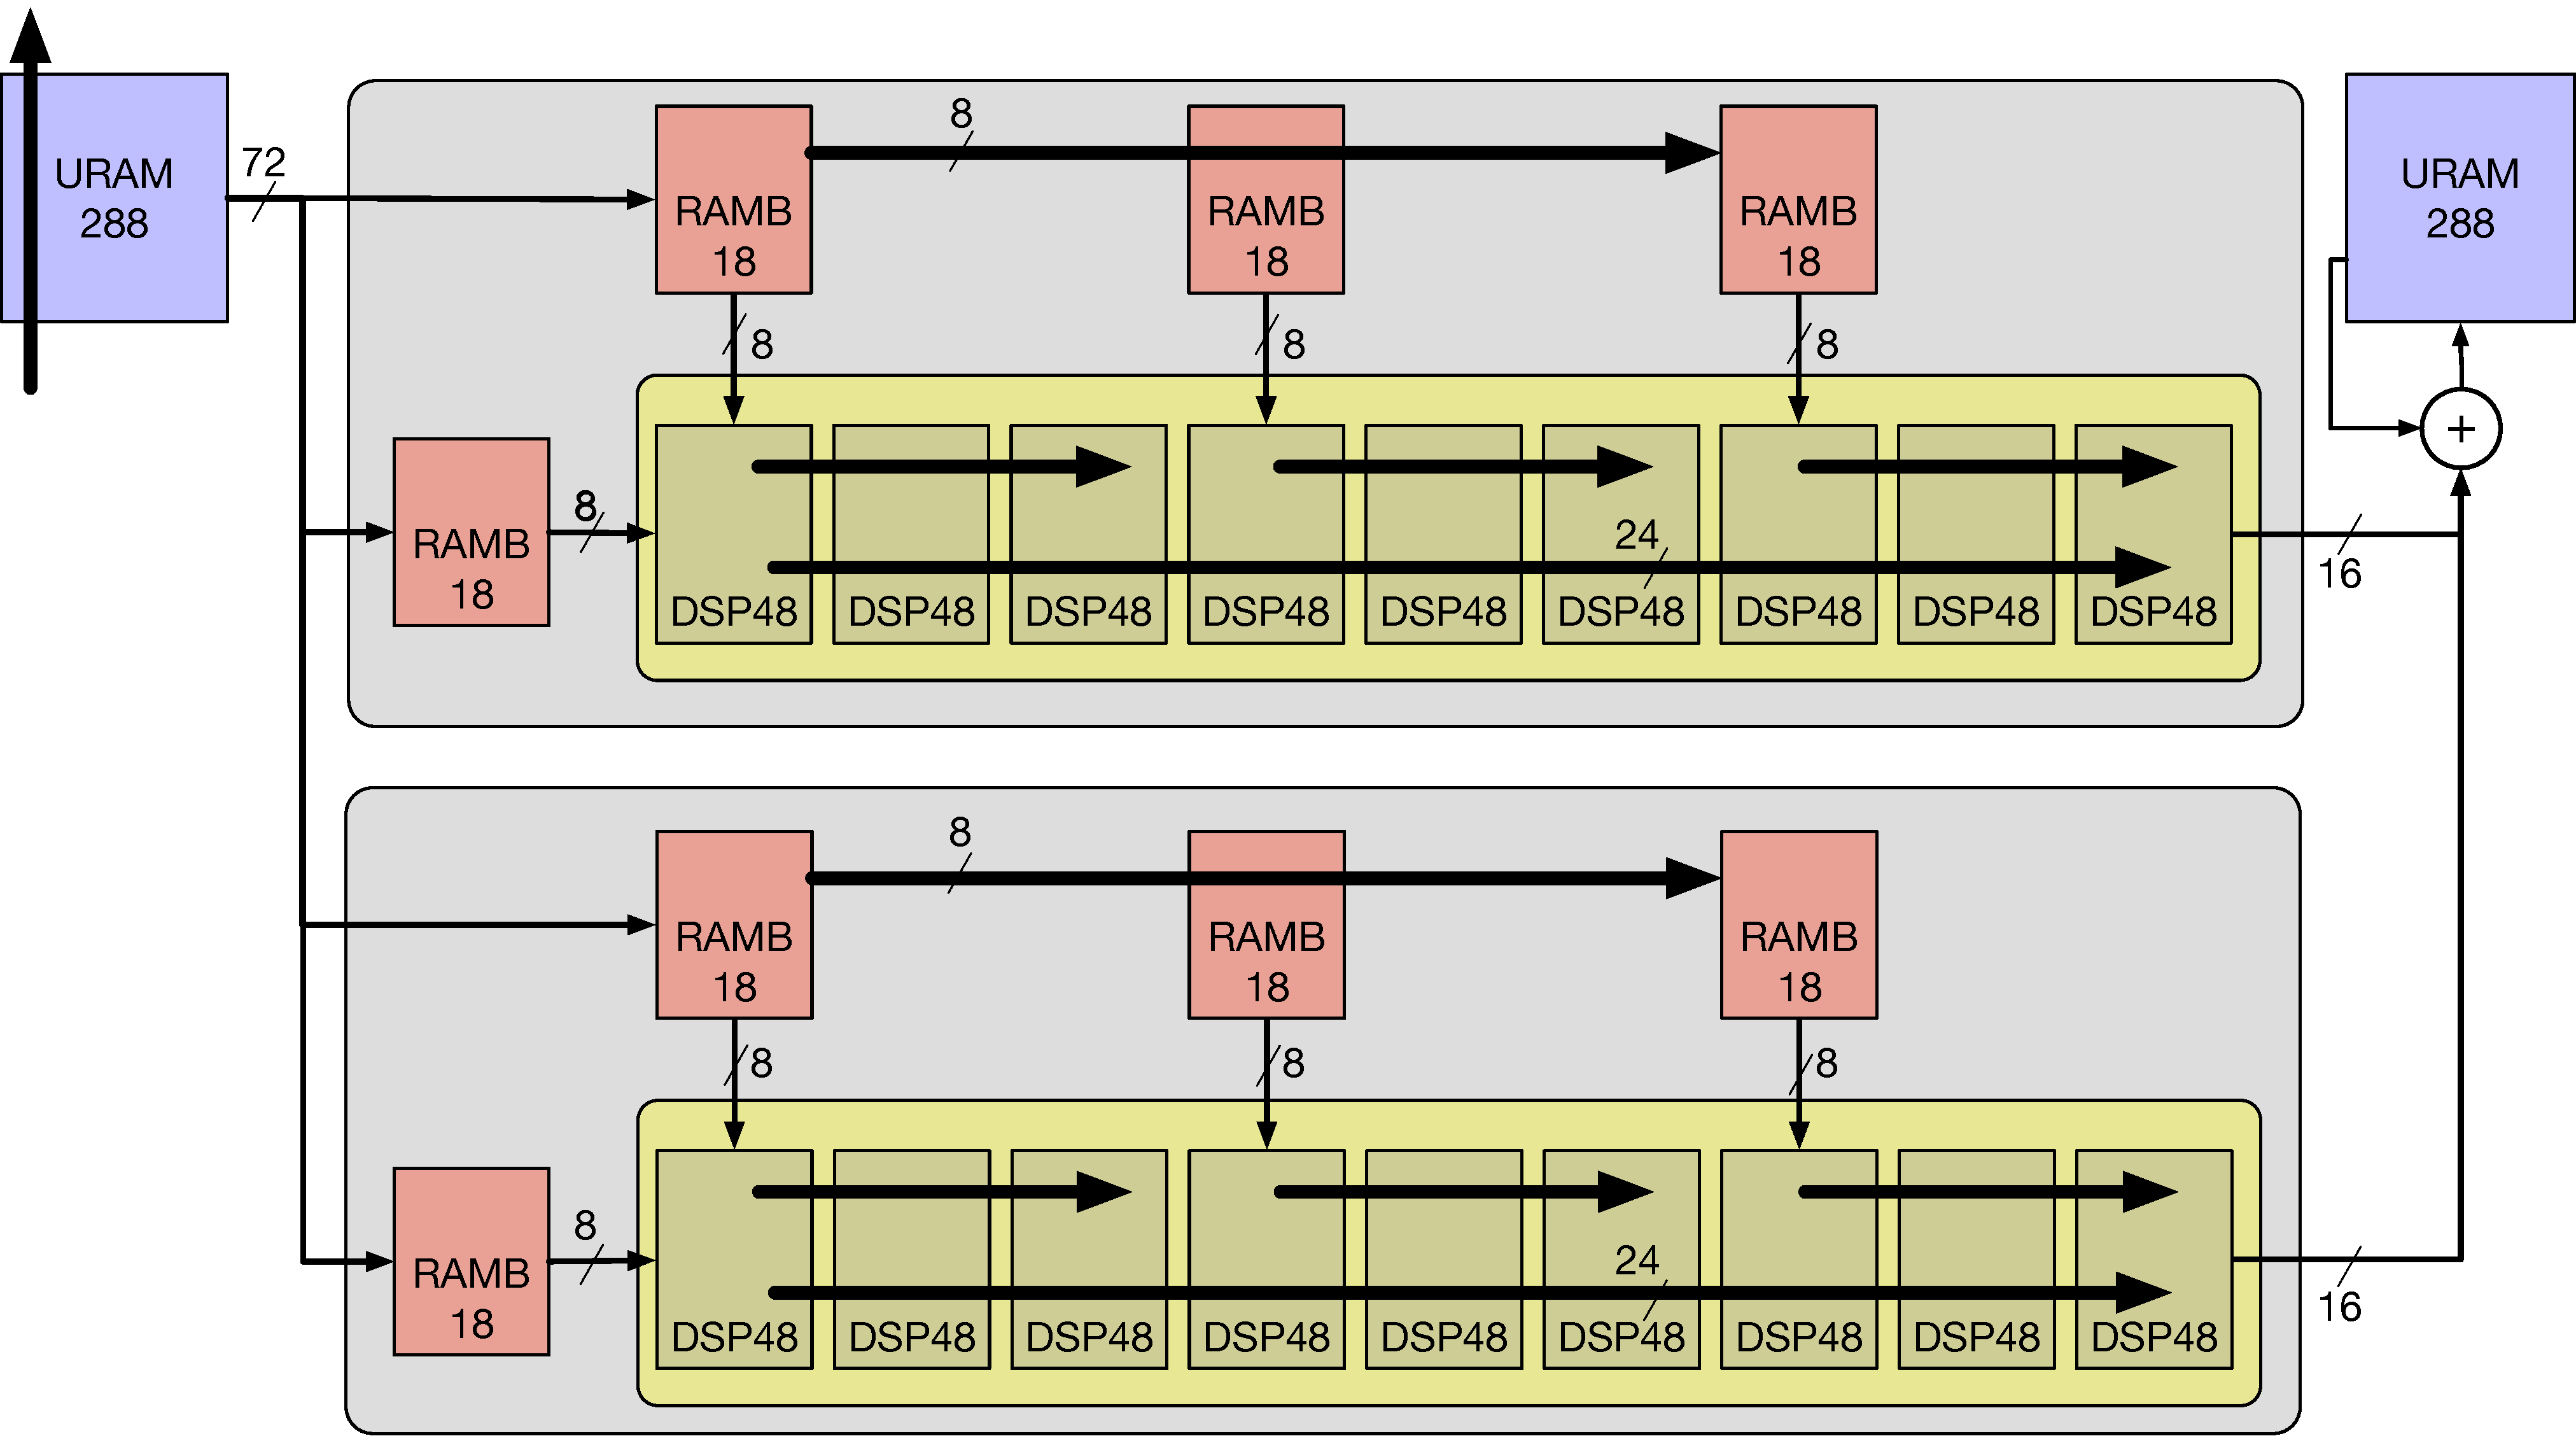
\includegraphics[width=0.8\textwidth]{figure/array}
	\caption{脉动阵列卷积计算单元~\cite{nachiket_stc_fpl2019}} 
	\label{fig:sys}
\end{figure}


\begin{figure}[h]
	\centering
	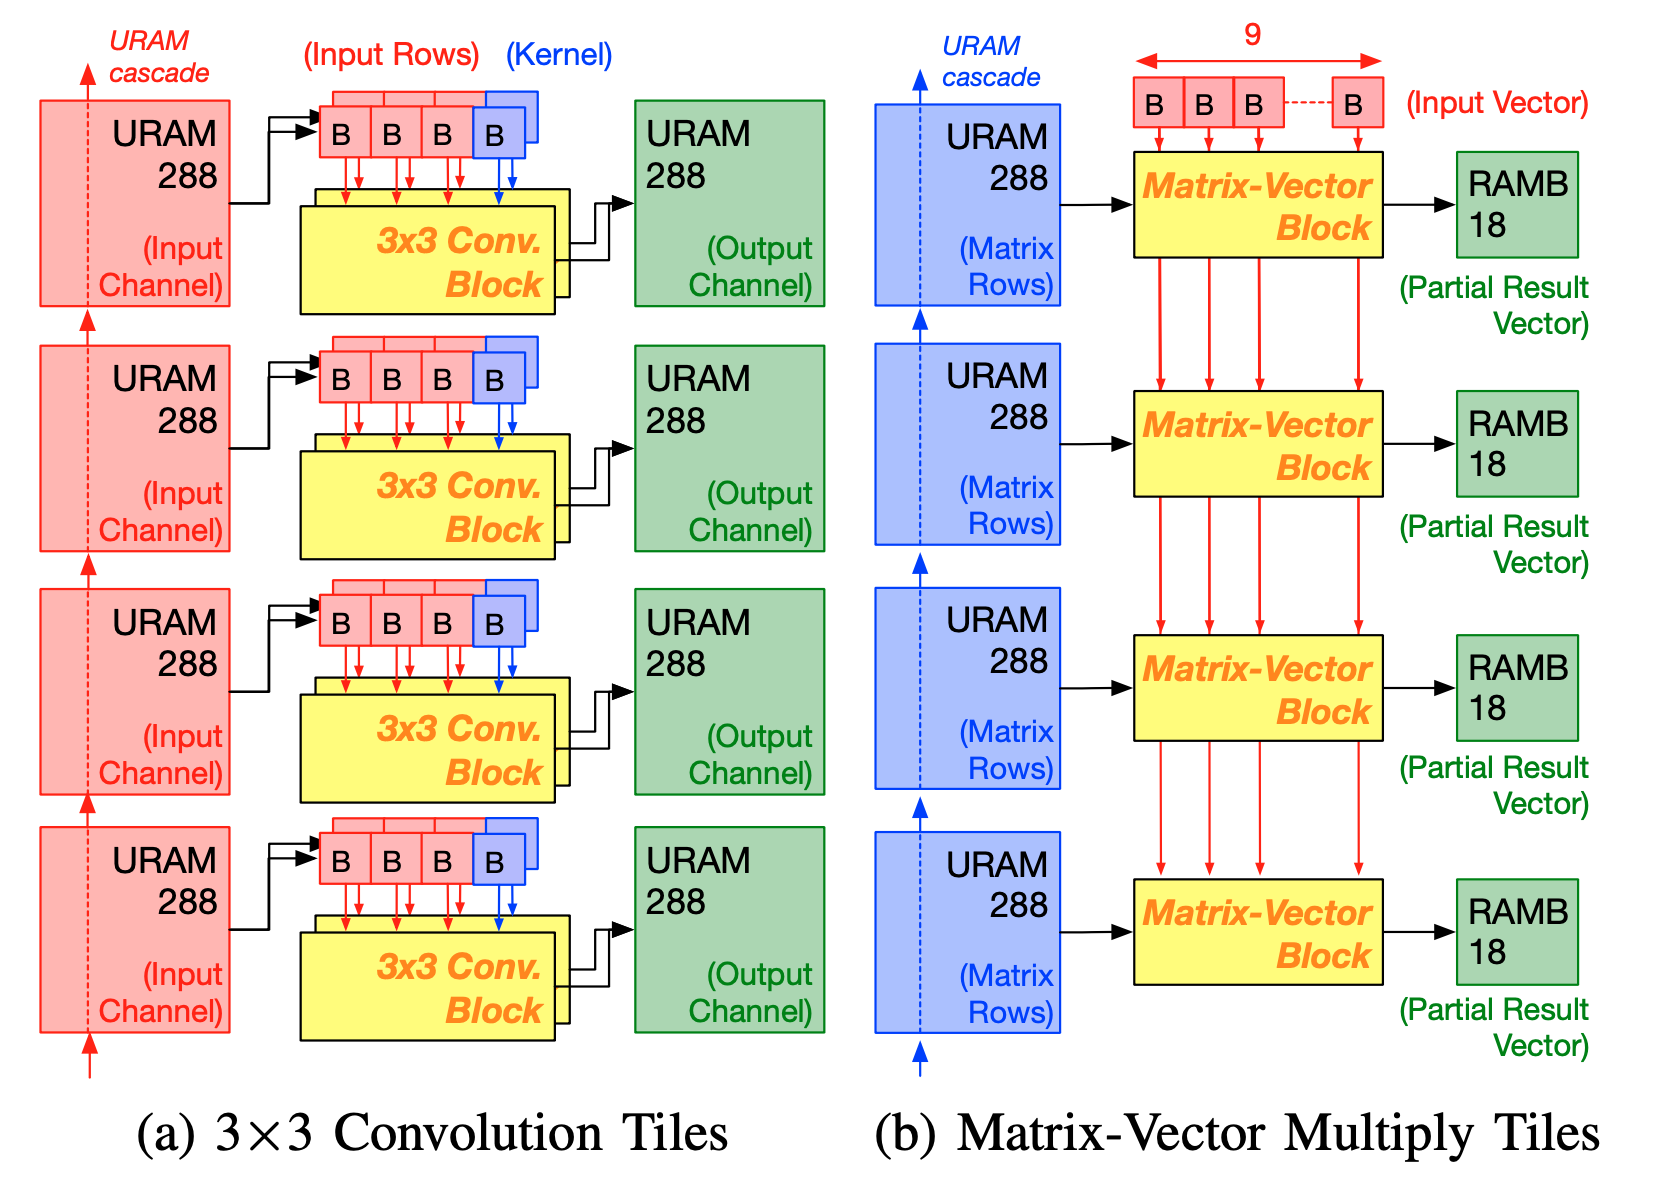
\includegraphics[width=0.8\textwidth]{figure/cascade}
	\caption{卷积运算单元和矩阵乘法运算单元级联的脉动阵列~\cite{nachiket_stc_fpl2019}} 
	\label{fig:cas}
\end{figure}

图\ref{fig:sys}为Scale and Cascade~\cite{nachiket_stc_fpl2019}提出的脉动阵列卷积计算单元架构图。一个卷积计算单元由2个Ultra RAM,8个Block RAM,
18个DSP48构成。其中输入URAM用于存储特征图的两个通道,和一个卷积核的权重。URAM连接着两组乘加计算单元,每一组分别有3个BRAM负责
移位寄存特征图像素,1个BRAM存储卷积核权重。在乘加计算单元里权重和特征像素不断由BRAM输送给级联的DSP48,在这里计算乘积并将
结果累加。最后一个DSP输出的值就是一次卷积的计算结果,并由输出端的URAM存储。此设计的并行度为2倍卷积核行数,但特征图像素数据复用更高,
同时时钟频率相比Line-Buffer设计更高,更适合大规模神经网络加速。

图\ref{fig:cas}说明了卷积单元和矩阵乘法单元级联组成脉动阵列的方式。矩阵乘法单元的设计与卷积类似,不同之处在于乘加单元中BRAM数目增加到
9个,计算结果由一个BRAM存储。URAM的级联同时增加了特征图的通道复用,进一步提高了设计的并行度。

\section{FPGA EDA实现原理}

FPGA设计的EDA实现过程主要分为5个部分~\cite{li2017utplacef}:合成(Synthesis),工艺映射(Technology Mapping),打包(Packing),布局(Placement),布线(Routing)。
本节分别对每个步骤进行阐述。
\begin{figure}[h]
	\centering
	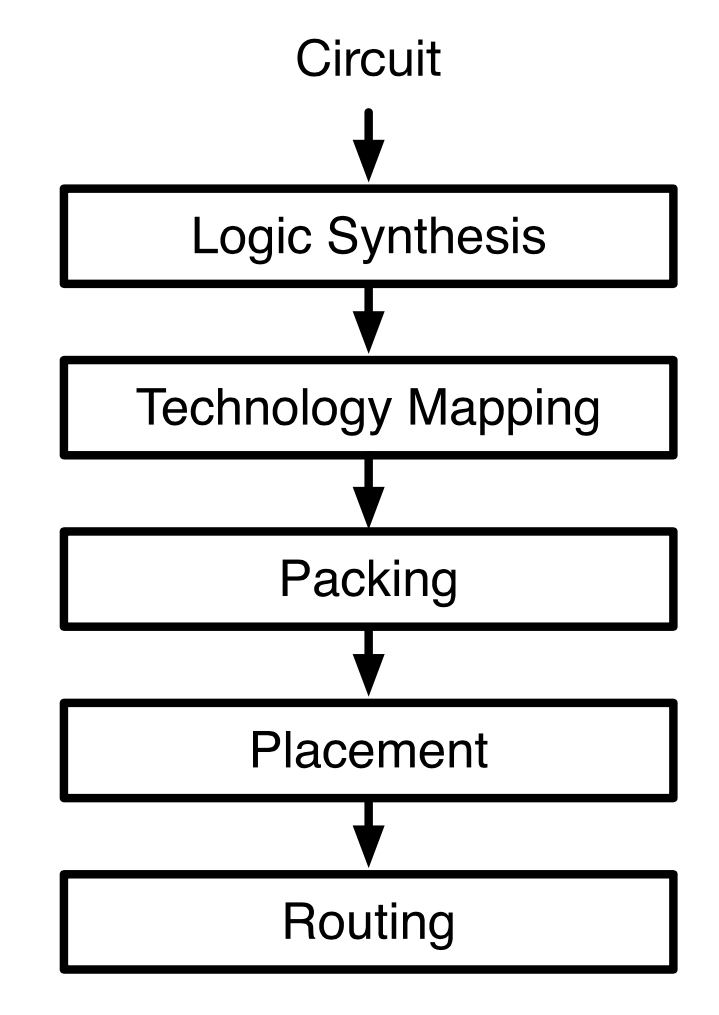
\includegraphics[width=0.3\textwidth]{figure/cad}
	\caption{FPGA设计的EDA实现步骤~\cite{li2017utplacef}} 
	\label{fig:eda}
\end{figure}
\begin{itemize}
    \item 合成和工艺映射:在这两个步骤中,电路设计编译和转化为逻辑网表,网表中通常包括信号线与LUT和Flip-Flop。
    \item 打包:此步骤将上一步产生的网表进行打包,将LUTs和Flip-Flop打包成CLB(Configurable Logic Block)。经过打包阶段的逻辑网表
    可以与FPGA上的计算单元相对应,可用于后续的布局布线。
    \item 布局: 布局阶段为打包之后的逻辑网表中的逻辑单元确定对应的物理位置,同时优化某些目标,比如最小化阻塞、线长等,目的是在于
    产生可以布线的布局结果,同时尽可能满足时序要求。
    \item 布线:将布局之后的电路根据信号线连接起来。在FPGA中横向或纵向的连接是通过PIP(Programmable Interconnect Points)完成的,
    而横向与纵向的连接通过switch box完成。这一阶段也包括时钟信号的连线。经过布线的设计可以产生时序报告,得到最高运行时钟频率。
\end{itemize}

\section{RapidWright FPGA实现框架}
                                                                                                                                                                                                                                                                                                                                                                                                                                                                                                                                                                                                                                                                                                                                                                                                                                                                                                                                                                                                                                                                                                                                                                                                                                                                                                                                                                                                                                                                                                                                                                                                                                                                                                                                                                                                                                                                                                                                                                                                                                                                                                                                                                                                                                                                                                                                                                                                                                                                                                                                                                                                                                                            
\begin{figure}[h]
	\centering
	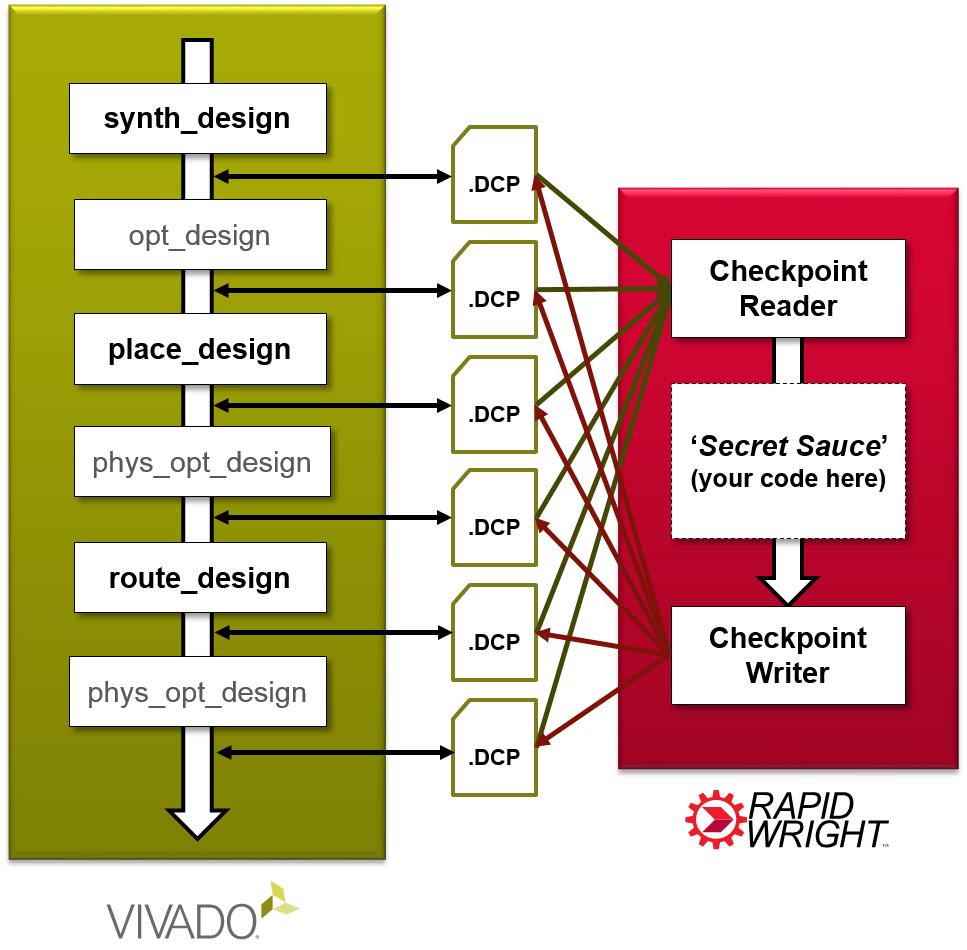
\includegraphics[width=0.8\textwidth]{figure/vivado_dcps}
	\caption{RapidWright FPGA实现框架~\cite{lavin2018rapidwright}} 
	\label{fig:rapidwright}
\end{figure}

\subsection{RapidWright简介}

RapidWright~\cite{lavin2018rapidwright}是Xilinx Research Lab 开发的开源Java FPGA自定义框架,能够修改基于 Xilinx FPGA 和 SoC 的逻辑网表设计
与物理实现修改,它提供了 Xilinx Vivado Design Suite 许多功能的补充,其中包括:
\begin{itemize}
    \item 快速加载和浏览Vivado支持的Xilinx设备物理模型;
    \item 导入和写出未加密的DCP checkpoint文件;
    \item 精确修改FPGA设计的逻辑网表和物理实现,如修改布局和布线;
    \item 提供一种模块化的快速实现方法,可将先前实现的设计作为新设计中的一个模块,对其修改、复制或迁移位置。
\end{itemize}

RapidWright的优势在于它与Vivado的完全兼容性,对Xilinx FPGA设备物理信息的快速获取能力和精确修改设计的能力。其基于Java的实现
为许多创新性任务带来了便捷,比如通过RapidWright可以精确获得FPGA器件上某一个元件的位置、它在设计中的状态:是否被用于布局,是否完成
布线等信息,甚至具体到每个可编程连接点(PIP)和信号线的状态都可精确获知。RapidWright支持Vivado TCL Interface的全部功能,
同时提供更高的操作精确度和更便捷的获取方法。

\subsection{DCP简介}

图\ref{fig:rapidwright}为Vivado与RapidWright的交互方式。在Vivado合成到布线中间的每一个过程中,都可将
设计导出为一个DCP格式的checkpoint文件,DCP文件中包含了该设计的逻辑网表、约束文件、物理网表实现结果与相应器件信息,可以完全确定
FPGA设计在该阶段的状态,因此DCP文件也包含设计的布局与布线信息。

RapidWright提供了快速的DCP文件读入和写出功能,一个完整的FPGA设计包括其逻辑网表、约束和布局布线信息都反映在RapidWright的
\texttt{Design}类中,在此基础上可以对其中的每一项通过RapidWright提供的API进行精确的修改。修改完毕的设计使用\texttt{Design}
类中的DCP写出API将修改后的设计导出为Vivado兼容的DCP格式,可以用Vivado打开、查看、继续修改,生成比特流。
RapidWright提供了一种面向对象的FPGA实现方法,实现的所有方面信息都有对应的类表示,在操作时使用该类的对象以及提供的API。


\section{FPGA计算架构构成}

FPGA(Field Programmable Gate Array,场可编程门阵列) 是一类可以通过编程方法修改其内部逻辑的芯片。早期的FPGA大多包含由
SRAM实现的可编程逻辑模块和IO模块,每个可编程逻辑模块中包含查找表和寄存器。而现代FPGA除了可编程模块加入了多种新型IP核,比如
片上分布式RAM,DSP模块,PCIe模块等等。本节首先介绍FPGA的几种基本组成元件,然后以Xilinx FPGA为例,介绍现代异构FPGA的
组成结构,并详细介绍UltraScale+系列配备的IP硬核~\cite{ug903}。

\subsection{FPGA的基本组成元件}

{\bf LUT}

LUT(查找表)是FPGA可编程逻辑的核心,也是计算的基本组成单元。LUT一般是多输入、单输出的,输出信号通过输入选择信号和存储器的
内容确定。目前常用的LUT一般是6个输入信号。

\begin{figure}[h]
	\centering
	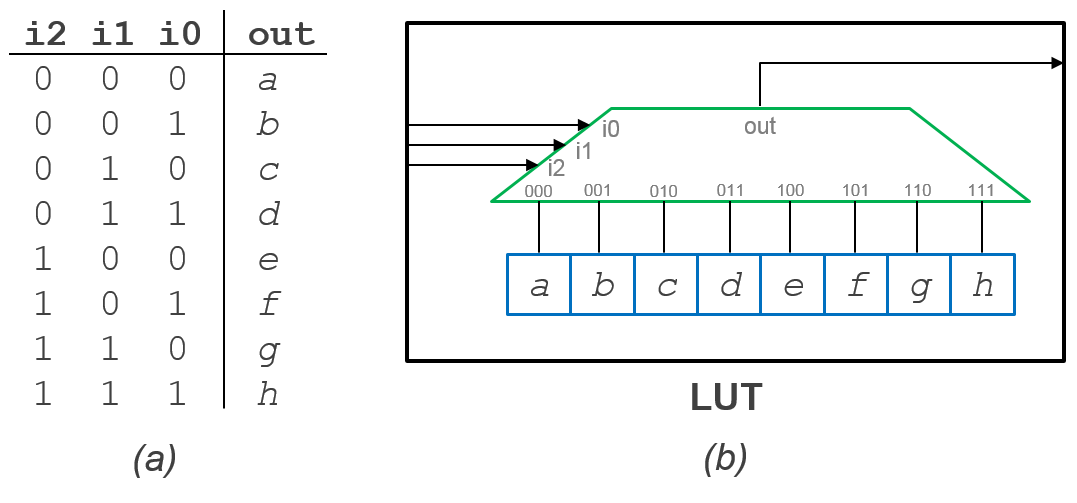
\includegraphics[width=0.7\textwidth]{figure/luts}
	\caption{FPGA的基本组成元件:查找表LUT与真值表的关系~\cite{lavin2018rapidwright}} 
	\label{fig:lut}
\end{figure}

图\ref{fig:lut}展示了一个三输入LUT的例子。LUT通常以 N:1 选择器和一个 N 比特存储器的形式实现,在图\ref{fig:lut}的例子中
N=8,如果输入比特数为$k$,则 $N=2^k$。LUT能够实现任意$k$输入单输出的逻辑函数,这是因为LUT与真值表的对应关系。输入信号用于
多路选择器的信号选择,而真值表对应输入的输出值则通过存储器存在多路选择器的对应位置中,这样每次仅需修改存储器中的值就可实现
任意逻辑函数,这也就是FPGA计算可编程性的来源。

{\bf State Element}

LUT的计算值输出后通常需要寄存。因此大多数的FPGA将LUT和 D-Flip Flop 连接为一组逻辑,称为状态单元(State Element)。通常来说
这里的寄存单元使用reset/clear信号和时钟来确定工作方式,并可以作为锁存器使用,这些状态单元通常都有专用的时钟路径。FPGA将任意数量
的状态单元连接起来,就可以实现任意的逻辑函数。Xilinx提供一种基于LUT的状态单元变种,支持在LUT的存储器单元内寄存数据,这样的LUT可以
通过编程当做小型存储、移位寄存器或FIFO使用。

{\bf Carry Chain}

Carry Chain 是FPGA的基本组成元件之一,通常一组LUT会配备一个Carry Chain来实现高效的可编程逻辑。Carry Chain 一般用于简单
逻辑操作的专用进位通道,比如加法、减法、比较等等。虽然Carry Chain 的功能可用LUT实现,但专用的进位通道对资源的利用更加高效,
性能也更好。

{\bf DSP}

在FPGA上直接用LUT实现乘法器是非常昂贵的,同时乘法又是极为普遍的运算之一,因此许多现代FPGA专门设计了乘法计算单元。这些乘法
计算单元一般是专用的IP硬核,支持整数乘法操作。随着FPGA的进化更先进的DSP也支持乘累加操作和宽位AND/XOR操作等等。

{\bf Block RAMs}

现代FPGA通常在片上设置大型的存储器,可以达到几十KB。这些存储器在片上通常是分布式的,并且使用非常灵活,支持单/双口读写,
拆分或者级联。以Xilinx UltraScale+架构为例,此系列FPGA提供两类Block RAM,一类是BRAM,另一类是更大的URAM。



\subsection{现代异构FPGA的组成架构}

本小结以Xilinx架构为例阐述现代FPGA的组成结构。对于Xilinx FPGA 来说,其架构主要分为6级,从最基本的可编程单元
一直到整个FPGA。图\ref{fig:hierarchy}描述了该6个级别。

\begin{figure}[h]
	\centering
	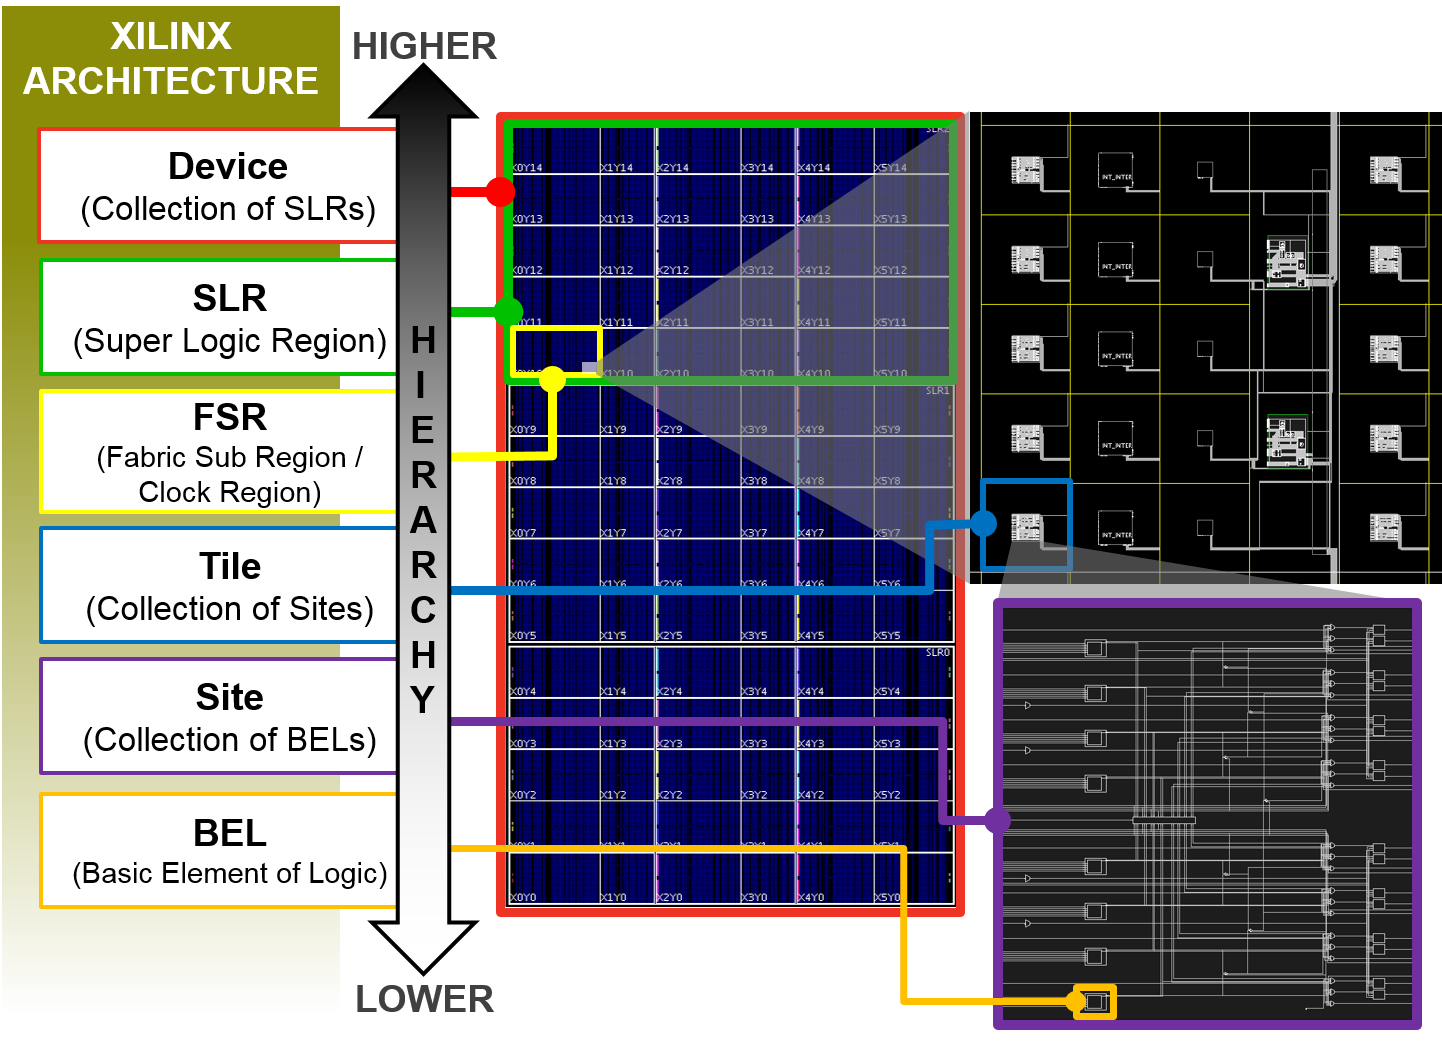
\includegraphics[width=0.8\textwidth]{figure/hierarchy}
	\caption{Xilinx FPGA 可编程硬件组成结构~\cite{lavin2018rapidwright}} 
	\label{fig:hierarchy}
\end{figure}

{\bf BEL: Basic Element of Logic}

BEL是Xilinx FPGA 最小的物理计算单元。BEL分为两类,一类是Logic BEL,另一类是Routing BEL。Logic BEL实际上就是包含
LUT,FF等在内的最小逻辑计算单元,实现逻辑计算。将逻辑网表中的叶节点对应到Logic BEL上,就是“布局”的含义。
Routing BEL是可编程的多路选择器,用来编程连通或断开Logic BEL 之间的连接,也就是布线。以Routing BEL为基础的
布线资源称为PIP,Programmable Interconnect Point。

{\bf Site}

一组有连接关系的BEL聚集在一起构成了一个Site,在Site中有三种元件:BEL,Site Pin 和 Site Wire。Site Pin 用于
连接内部元件和外部资源,也就是引脚。Site Wire 负责连接内部各个BEL和Site Pin。在Xilinx FPGA架构中,每一个Site有
自己的位置编号,不同种类的Site单独编号,因此可以方便地找出其相对位置或用于索引。

{\bf Tile}

Tile是构建FPGA的模块,一个Tile可包含多个Site,但也可以不包含任何Site。Tile内部和之间的连线是通过PIP实现的Node完成的。
Node是延伸多个Tile的电路连接,从Node的连接状态可以获知其初始点与终点,以及连接中间经过的Tile。Xilinx FPGA 使用一种
列主导的Tile构建方式,也就是同一列的Tile一般是相同类型的。

{\bf FSR: Fabric Sub Region}

FSR就是通常所说的时钟域,其中包含多个Tile,各自有独立的时钟资源。在Xilinx UltraScale架构中,FSR的高度都相同,而
宽度根据不同的内部构成有所不同。


{\bf SLR: Super Logic Region}

SLR也称为超逻辑域,其出现始于FPGA 2.5D Packaging 工艺的发展。现代大型FPGA一般包含多个硅片,每一个单独的硅片就是
一个SLR,可看作一个完整的独立芯片。SLR一般包含多个时钟域,其边缘与其他SLR的连接通过专用的跨逻辑域通路,并有专用的
Tile辅助跨逻辑连接,叫做 Laguna Tiles~\cite{ug903}.


{\bf Device}

Xilinx FPGA架构中最高级别的架构是Device,代表整个FPGA,一般由一个或多个SLR纵向堆叠构成。






\subsection{UltraScale+ IP硬核介绍}

Xilinx UltraScale+ 系列FPGA集成了上千个IP硬核(hard block),这些硬核具有高时钟频率,高性能,
可配置等特点,本小结详细阐述三种IP硬核的特点。

\begin{figure}[h]
    \centering
	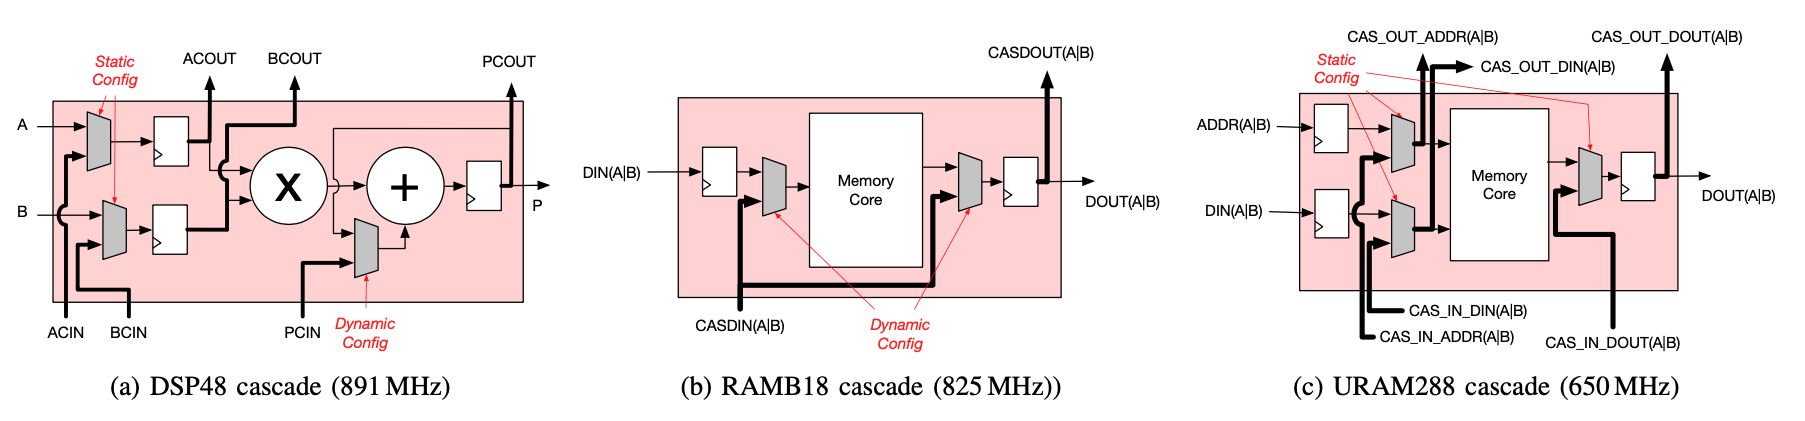
\includegraphics[width=\textwidth]{figure/hardblocks}
	\caption{Xilinx UltraScale+ IP硬核介绍~\cite{nachiket_stc_fpl2019}} 
	\label{fig:hardblocks}
\end{figure}

\begin{itemize}
    \item {\bf DSP48E2} (图\ref{fig:hardblocks} a)
    支持$27\times18$整数乘法,48位累加。Xilinx DSP48支持的最高时钟频率为891 MHz,并且支持
    功能选择。DSP48不仅可以配置运算类型,还可以改变数据通路。因此,本文的脉动阵列设计利用
    DSP48E2可选数据通路和支持级联的特性将DSP48E2设置为MAC(Multiply and Accumulate)功能,
    并且串流输入数据进行复用。
    
    \item {\bf RAMB18} (图\ref{fig:hardblocks} b)
    Xilinx FPGA 集成数千个分布式块存储器,其输入输出位宽可以配置。RAMB18最高支持时钟频率
    为825 MHz,并且提供特殊的级联配置。RAMB18允许用于将邻近的多个BRAM级联成为一个更深的
    存储器或者FIFO。本文利用RAMB18的级联特性进行卷积设计中的特征图数据复用。
    
    \item {\bf URAM288} (图\ref{fig:hardblocks} c)
    UltraScale+独有的超大型片上存储器Ultra RAM,也就是URAM288.URAM288支持288kb存储,
    其位宽不可配置,但仍支持级联配置。URAM288支持的最高时钟频率为650 MHz。在实际布局问题中,
    本文的优化目标就是使布线后的完整脉动阵列加速器时钟频率不低于650 MHz。

\end{itemize}



\section{FPGA布局算法}

FPGA布局问题是将打包后的逻辑网表中的元件对应到FPGA物理位置的过程,其目标是寻找对应关系的同时优化特定目标,比如
设计可布线性,关键路径长度或阻塞程度。
FPGA布局已被证实为NP-complete问题~\cite{panchal2015solving},且FPGA的布局结果直接影响设计是否可布线以及实现后的时序表现,因此布局是
EDA问题中的重点和难点。本节通过总结已有的和近年发展的FPGA布局方法从整体角度阐述FPGA布局算法原理。


FPGA布局算法可基本分为四类:基于模拟退火的布局算法~\cite{eguro_retime,kirkpatrick1983optimization},进化类算法~\cite{yang2005fpga,venkatraman2000evolutionary,jamieson2013supergenes,wang2009ant},Min-Cut Partition~\cite{maidee2005timing},解析类布局算法\cite{gort_analytical-placement_fpl2012,abuowaimer2018gplace3}。

\subsection{模拟退火}
模拟退火法出现较早且应用广泛,经过随机初始化的布局在温度函数的控制下逐渐降低接受随机变化的概率,使系统冷却,从而得到最优布局结果。
基于模拟退火法的布局工具VPR在学术界获得认可,其改进的目标函数广泛适用于各种架构和电路设计布局。
退火法得到的布局结果质量高,但所需迭代优化时间较长,并行度和可扩展性较差。另外,退火法的结果受其温度设定影响较大。
退火的温度函数也称为冷却进度表,其规定退火的初始温度,下降速率等信息。冷却过快会导致系统无法充分收敛,最终
的优化结果较差;冷却过慢则导致收敛时间过长,无法在可行时间范围内给出最优解。因此,退火法需要人工调节参数,
收敛速度与结果质量与具体优化设置高度相关。


\subsection{进化算法}
进化算法是一类受到达尔文进化论启发的优化算法,经典的例子包括遗传算法、蚁群算法、粒子群算法等等~\cite{DBLP:journals/corr/abs-1906-08870}。进化算法作为一种
迭代优化方法其核心思想在于使用基因型编码可行解,定义目标函数(或称为适应度函数),然后通过基因型的交叉、变异在迭代过程中
产生新的可行解,然后通过目标函数将适应度低的基因型或个体淘汰,以此使种群趋向于目标函数的方向进化。
一般认为,应用于FPGA布局的进化算法表现不如退火,其原因在于交叉算子对解空间探索性能较差。但进化算法基于种群进化的思想
具有适应并行化的优势,因为同一迭代周期内的个体可以同时计算适应度,不存在依赖关系;而退火下一次随机操作基于当前的状态,因此
不具有并行化的优势。而且,近年来人工智能和优化领域的发展推动了多目标和高鲁棒性进化算法的发展,并已在强化学习、神经网络
结构搜索等领域取得了领先的表现。因此,将现代进化算法应用于FPGA布局是具有前景的研究方向。

\subsection{Min-Cut Partition}
Min-Cut法将逻辑网表不断按区域划分,直到网表内元件完全展开
和FPGA物理位置对应,适用于小型布局问题,且局部优化容易收敛至局部最优。

\subsection{解析布局算法}
近年来获得较大发展的方法是解析布局法,其将FPGA布局优化问题建模为
方程系统,并使用求解算法解得布局结果。常用的求解算法如QP法(Quadratic Programming),通过求梯度求解目标函数的最小值。
解析布局算法可扩展性强,结果质量较高,但需要代价较大的布局结果合法化过程,可并行度较差。
目前广泛应用的Vivado Design Suite中使用的布局算法为多目标解析算法,优化目标为时钟频率,阻塞和线长~\cite{wp416-vivado-user-guide}。



\section{本章小结}

本章首先介绍了神经网络硬件加速的两种经典架构,然后阐述了FPGA EDA实现过程的基本步骤,明确了EDA中布局过程的重要性和挑战。接着
详细介绍了本文使用的FPGA实现工具RapidWright与Xilinx FPGA的计算架构。最后,本章介绍了目前主流的四类FPGA布局算法,分别阐述了
各自的基本原理、总结优势以及不足之处。


































































% \section{图像颜色编辑的梯度感知优化策略}
% 论文主体是毕业论文的主要部分,必须言之成理,论据可靠 \cite{tighe2013finding},严格遵循本学科国际通行的学术规范。
% 在写作上要注意结构合理、层次分明、重点突出。

% 本章举例说明本模板中图片,表格及公式的插入及引用方法 \cite{liu2011sift}。

% \subsection{图片格式举例}

% 图片的分辨率至少300个像素,建议格式为.png。图 \ref{fig1} 显示……,图 \ref{subfig1} 表明……。

% \subsubsection{单张图片}
% \begin{figure}[h]
% 	\centering
% 	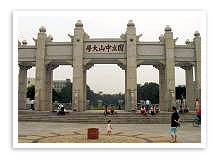
\includegraphics[width=0.8\textwidth]{figure/fig1.png}
% 	\caption{标题} 
% 	\label{fig1}
% \end{figure}

% \subsubsection{多张子图}
% \begin{figure}[h!] % image examples & compare
% 	\begin{subfigure}{0.55\textwidth}
% 		\centering
% 		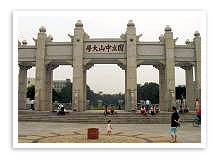
\includegraphics[width=0.5\textwidth]{figure/fig1.png}
% 		\caption{子图1}
% 		\label{subfig1}
% 	\end{subfigure}
% 	\begin{subfigure}{0.55\textwidth}
% 		\centering
% 		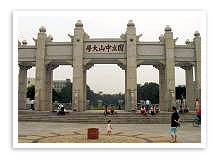
\includegraphics[width=0.5\textwidth]{figure/fig1.png} 
% 		\caption{子图2}
% 		\label{subfig2}
% 	\end{subfigure}
% 	\begin{subfigure}{0.55\textwidth}
% 		\centering
% 		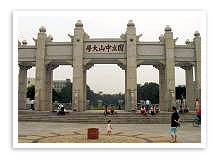
\includegraphics[width=0.5\textwidth]{figure/fig1.png}
% 		\caption{子图3}
% 		\label{subfig3}
% 	\end{subfigure}
% 	\begin{subfigure}{0.55\textwidth}
% 		\centering
% 		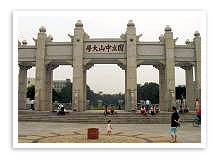
\includegraphics[width=0.5\textwidth]{figure/fig1.png} 
% 		\caption{子图4}
% 		\label{subfig4}
% 	\end{subfigure}
% 	\caption{多子图}
% 	\label{subfig}
% \end{figure}




% \subsection{表格举例}
% 表 \ref{tab1} 表示……。
% \begin{table}[h]
% 	\centering
% 	\caption{国际单位制中具有专门名称的导出单位}		
% 	\label{tab1}
% 	\begin{tabular}{c|c|c|c}
% 		\toprule[2pt]
% 		量的名称 & 单位名称 & 单位符号 & 其他表示式例\\
% 		\midrule[2pt]
% 		频率	& 赫[兹]	& Hz	&$s^{-1}$ \\
% 		\hline                                        %细横线
% 		力;重力 	& 牛[顿]	& $N$	 & $kg·m/s^2$ \\
% 		\hline                                         %细横线
% 		压力,压强;应力	& 帕[斯卡]	&$Pa$	&$N/m^2$ \\
% 		\bottomrule[2pt]
% 	\end{tabular}
% \end{table}

% \subsection{公式举例}
% \label{sec:formula}
% 没有编号的公式:
% \begin{equation*}
% \bm{z}^{(l)} = \bm{W}^{(l)}\bm{a}^{(l-1)} + \bm{b}^{(l)} 
% \end{equation*}

% 公式中含有中文:
% \begin{equation}
% \mbox{像素准确率} = \sum_{i=1}^{n_{cl}}n_{ii} / \sum_{i=1}^{n_{cl}}t_i
% \end{equation}

% 公式中含有矩阵:
% \begin{equation}
% \label{eq1}
% \textbf{H} = \begin{bmatrix}
% I*\bm{x}_i \\ \textbf{h}
% \end{bmatrix}
% \end{equation}

% 多行公式:
% \begin{align} 
% \hat{\bm{R}}_r 
% & =   \frac{1}{N_s} \sum_{i=1}^{Ns} \bm{r}_i \bm{r}_i^T  \label{Eq-2-a} \\
% & =   \frac{1}{N_s} \sum_{i=1}^{Ns} \bm{r}_i \bm{r}_i^T  \nonumber \\
% & =   \frac{1}{N_s} \sum_{i=1}^{Ns} \bm{r}_i \bm{r}_i^T  \label{Eq-2-c},
% \end{align}

% 引用:公式 \eqref{eq1} ……,\eqref{Eq-2-a}……。

% 更多的数学公式编辑方法,请参考根文件下“LaTex学习文档”中的文献1和文献3。

% \subsection{算法举例}


% \begin{algorithm}[h]
% 	\KwIn{$m$个训练样本}
% 	\lFor{$l=1$ \emph{\KwTo} $n_l$}{
% 		初始化:$\Delta \bm{W}^{(l)}=0$,$\Delta \bm{b}^{(l)}=0$}
% 	\ForEach{训练样本}{
% 		\lFor{$l=1$ \emph{\KwTo} $n_l-1$}{
% 			前向传播:$\bm{z}^{(l+1)}=\bm{W}^la^l+\bm{b}^l$,$\bm{a}^{(l+1)}=f(\bm{z}^{(l+1)})$}
% 		输出误差计算:$\delta^{(n_l)} = \frac{\partial}{\partial \bm{z}^{(n_l)}} J(\bm{W},\bm{b};\bm{x},y)$\;
% 		\lFor{$l=n_l-1$ \emph{\KwTo} $1$}{
% 			后向传播:$\delta^{(l)} = \bigl((\bm{W}^{(l)})^T \delta^{(l+1)}\bigr)f'(\bm{z}^{(l)})$}
% 		\ForAll{层l}{
% 			计算梯度:$\nabla_{\bm{W}^{(l)}}J(\bm{W},\bm{b};\bm{x},y)=\delta^{(l+1)}(\bm{a}^{(l)})^T$ \\
% 			\hspace{60pt}$\nabla_{\bm{b}^{(l)}}J(\bm{W},\bm{b};\bm{x},y)=\delta^{(l+1)}$\;
% 			累加梯度:$\Delta \bm{W}^{(l)} \leftarrow \Delta \bm{W}^{(l)} + \nabla_{\bm{W}^{(l)}}J(\bm{W},\bm{b};\bm{x},y)$; \\
% 			\hspace{60pt}$\Delta \bm{b}^{(l)} \leftarrow \Delta \bm{b}^{(l)} + \nabla_{\bm{b}^{(l)}}J(\bm{W},\bm{b};\bm{x},y)$\;
% 		}
% 	}
% 	\ForAll{层$l$}{
% 		更新权重:$\bm{W}^{(l)} \leftarrow \bm{W}^{(l)} - \alpha \biggl[\frac 1m \Delta \bm{W}^{(l)}]$ \\
% 		\hspace{60pt} $\bm{b}^{(l)} \leftarrow \bm{b}^{(l)} - \alpha \biggl[\frac 1m \Delta \bm{b}^{(l)}\biggr]$
% 	}
% 	\caption{梯度下降算法}
% 	\label{sgd}
% \end{algorithm}

% 算法 \ref{sgd}……。

% \subsection{例子}
% \begin{eg}
% 	这是一个例子。
% 	\label{eg1}
% \end{eg}
% 例 \ref{eg1} ……。

% \subsection{证明}
% \begin{proof}
% 证明过程
% \end{proof}

% \subsection{定理}
% \begin{theorem}
% 	这是一个定理。
% 	\label{th1}
% \end{theorem}
% 定理 \ref{th1} ……。

% \subsection{命题}
% \begin{proposition}
% 	这是一个命题。
% 	\label{pro1}
% \end{proposition}
% 命题 \ref{pro1} ……。

% \subsection{引理}
% \begin{lemma}
% 	这是一个引理。
% 	\label{lem1}
% \end{lemma}
% 引理 \ref{lem1} ……。

% \subsection{推论}
% \begin{corollary}
% 	这是一个推论。
% 	\label{cor1}
% \end{corollary}
% 推论 \ref{cor1} ……。

% \subsection{定义}
% \begin{definition}
% 	这是一个定义。
% 	\label{def1}
% \end{definition}
% 定义 \ref{def1} ……。

% \subsection{标记}
% \begin{remark}
% 	这是一个标记。
% 	\label{rem1}
% \end{remark}
% 标记 \ref{rem1} ……。


% \section{基于N维颜色直方图匹配的颜色映射方法}

% \section{梯度感知的颜色分布映射方法}

% \section{梯度感知的颜色分布映射方法实验结果分析}

% \section{本章小结}